\documentclass[french]{article}
\usepackage[T1]{fontenc}
\usepackage[utf8]{inputenc}
\usepackage[french]{babel}
\usepackage{amsmath}
\usepackage{mathtools}
\usepackage{color}
\usepackage[svgnames,dvipsnames]{xcolor} 
\usepackage{soul}
\usepackage{amssymb}
\usepackage{enumitem}
\usepackage{multicol}
\usepackage[left=2cm,right=2cm,top=2cm,bottom=2cm]{geometry}
\newcommand{\mathcolorbox}[2]{\colorbox{#1}{$\displaystyle #2$}}
\usepackage{pifont}
\usepackage{pst-all}
\usepackage{pstricks}
\usepackage{delarray}
\usepackage{setspace}
\usepackage{graphicx}
\usepackage{hyperref}
\usepackage{nicematrix}
\usepackage{listings}
\usepackage{float}

\hypersetup{
	colorlinks=true,
	linkcolor=blue,
	filecolor=magenta,      
	urlcolor=cyan,
	pdfpagemode=FullScreen,
}

\usepackage{amsthm}
\newtheorem*{Rem}{Remarque}

\newenvironment{conclusion}[1]{%
	\begin{center}\normalfont\textbf{Conclusion}\end{center}
	\begin{quotation} #1 \end{quotation}
}{%
	\vspace{1cm}
}

\lstset{language=C++,
	basicstyle=\ttfamily,
	keywordstyle=\color{blue}\ttfamily,
	stringstyle=\color{red}\ttfamily,
	commentstyle=\color{green}\ttfamily,
	morecomment=[l][\color{magenta}]{\#}
}

\setlength\parindent{0pt}

\begin{document}
	LECOURTIER Frédérique \hfill \today
	\begin{center}
		\Large\textbf{{Explication - Rehaussement avec FEM}}\\
	\end{center}
	\graphicspath{{images/}}

	On considère le problème de Poisson avec condition de Dirichlet homogène ou non homogène :
	\begin{equation}
		\label{pb1}
		\left\{\begin{aligned}
			&-\Delta u=f \quad &&\Omega \\
			&u=g \quad &&\Gamma
		\end{aligned}\right. \tag{$\mathcal{E}_1$}
	\end{equation}

	On a ainsi une EDP que l'on souhaite résoudre sur un domaine $\Omega$. On note $\Gamma$ le bord de $\Omega$, c'est-à-dire $\Gamma=\partial\Omega$. 
	
	Dans notre cas, on souhaite appliquer une correction à la sortie d'un FNO.
	On considère ici que l'on possède une solution analytique $u$ et qu'après une utilisation du FNO, on obtient une solution du type
	\begin{equation}
		\label{phi_tild}
		u_p(x,y) = u(x,y)-\epsilon P(x,y)
	\end{equation}
	avec $P$ la perturbation (tel que $P=0$ sur $\Gamma$) et $\epsilon$ petit.
	
	On supposera que $||P||_{H^{k+1}(\Omega)}\le 1$.
	
	On souhaite ainsi résoudre le problème suivant
	\begin{equation}
		\label{pb2}
		\left\{\begin{aligned}
			&-\Delta (\tilde{\phi}C)=f \quad &&\Omega \\
			&\tilde{u}=g \quad &&\Gamma
		\end{aligned}\right. \tag{$\mathcal{E}_2$}
	\end{equation}
	
	avec $\tilde{\phi}=u_p$ et $\tilde{u}=\tilde{\phi}C$.
	
	Ce document a pour but d'expliquer l'intérêt de rehausser la solution (avec FEM) afin de réduire le plus possible l'erreur $||u-u_{c}||_{L^2}$ où $u_{c}$ est la solution obtenu après la correction.
	
	\section*{Principe général de FEM}
	
	La démarche générale de la méthode des éléments finis consiste à écrire la formulation variationnelle de cette EDP et ainsi à se ramener à un problème du type
	
	\begin{equation}
		\text{Trouver } u\in V \text{ tel que } a(u,v)=l(v), \;\forall v\in V \tag{$\mathcal{P}$}
	\end{equation}

	On définit alors un maillage du domaine $\Omega$, grâce auquel on va définir un espace d'approximation $V_h$, sous-espace vectoriel de $V$ de dimension fini $N_h$. On écrit alors le problème approché

	\begin{equation}
		\text{Trouver } u_h\in V_h \text{ tel que } a(u_h,v_h)=l(v_h), \;\forall v_h\in V \tag{$\mathcal{P}_h$} \label{eq:pb_approach}
	\end{equation}

	On considère une base $(\varphi_1,\dots,\varphi_{N_h})$ de $V_h$. En décomposant $u_h$ sur cette base sous la forme
	
	\begin{equation}
		\label{decomp1}
		u_h=\sum_{i=1}^{N_h}\mu_i\varphi_i	
	\end{equation}
	
	le problème (\ref{eq:pb_approach}) se réécrit 
	
	\begin{equation*}
		\text{Trouver } \mu_1,\dots,\mu_{N_h} \text{ tels que } \sum_{i=1}^{N_h}\mu_i a(\varphi_i,v_h)=l(v_h), \;\forall v_h\in V 
	\end{equation*}

	ou encore
	
	\begin{equation*}
		\text{Trouver } \mu_1,\dots,\mu_{N_h} \text{ tels que } \sum_{i=1}^{N_h}\mu_i a(\varphi_i,\varphi_j)=l(\varphi_j), \;\forall j\in \{1,\dots,N_h\}
	\end{equation*}
	
	La résolution de l'EDP consiste alors à résoudre le système linéaire suivant :
	$$A\mu=b$$
	avec
	$$A=(a(\varphi_i,\varphi_j))_{1\le i,j\le N_h}, \quad \mu=(\mu_i)_{1\le i\le N_h} \quad \text{et} \quad b=(l(\varphi_j))_{1\le j\le N_h}$$
	
	Le théorème de convergence de FEM nous donne l'inégalité suivante :
	
	\begin{equation}
		||u-u_h||_{L^2(\Omega)}\le ch^{k+1}|u|_{H^{k+1}(\Omega)} \label{ine1}
	\end{equation}
	
	\section*{Application à la correction}
	
	On considère à présent uniquement le problème (\ref{pb2}). On peut alors effectuer le même type de raisonnement dans le cas de la correction. Ainsi par (\ref{decomp1}), la décomposition de $u_h$ sur la base $(\varphi_1,\dots,\varphi_{N_h})$ de $V_h$ s'écrit pour ce problème
	
	\begin{equation}
		u_h=\sum_{i=1}^{N_h}\mu_i(\varphi_i\tilde{\phi}(x))=\left(\sum_{i=1}^{N_h}\mu_i\varphi_i\right)\tilde{\phi}(x) \label{decomp2}
	\end{equation}
		
	Ainsi par (\ref{decomp2}) on en déduit
	$$\mu_i=\frac{u(x_i)}{\tilde{\phi}(x_i)}$$

	Et ainsi l'inégalité (\ref{ine1}) se réécrit pour le problème (\ref{pb2}):
	
	\begin{equation}
		\left|\left|\frac{u}{\tilde{\phi}}-C_h\right|\right|_{L^2(\Omega)}\le ch^{k+1}\left|\frac{u}{\tilde{\phi}}\right|_{H^{k+1}(\Omega)}||\tilde{\phi}||_{L^2(\Omega)} \label{ine2}
	\end{equation}

	avec $C=\frac{u}{\tilde{\phi}}$ la solution exacte au problème et $C_h$ la solution obtenue par FEM.
	
	\begin{Rem}
		On notera que si $\epsilon=0$ (c'est-à-dire qu'il n'y a pas de perturbation), alors $C=1$.
	\end{Rem}
	
	On considère une solution $\mathbb{P}^1$ ($k=1$), ainsi
	
	\begin{equation}
		\left|\frac{u}{\tilde{\phi}}\right|_{H^2(\Omega)}=\left|\left|\left(\frac{u}{\tilde{\phi}}\right)''\right|\right|_{L^2(\Omega)}=\epsilon\left|\left|\left(\frac{P}{\tilde{\phi}}\right)''\right|\right|_{L^2(\Omega)} \label{der1}
	\end{equation}
	
	car
	$$\left(\frac{u}{\tilde{\phi}}\right)''=\left(\frac{\tilde{\phi}+\epsilon P}{\tilde{\phi}}\right)''=\left(1+\epsilon\frac{P}{\tilde{\phi}}\right)''=\epsilon\left(\frac{P}{\tilde{\phi}}\right)''$$
	
	avec
	$$\left(\frac{P}{\tilde{\phi}}\right)''=\frac{P''\tilde{\phi}-P\tilde{\phi}''}{\tilde{\phi}^2}+\frac{2(P\tilde{\phi}'-P'\tilde{\phi})\tilde{\phi}'}{\tilde{\phi}^3}$$

	\section*{Rehaussement}
	
	L'idée du rehaussement est la suivante : on considère cette fois
	$$\hat{\phi}=\tilde{\phi}+m$$
	avec $m$ une constante.
	
	On souhaite alors résoudre le problème suivant
	
	\begin{equation}
		\left\{\begin{aligned}
			&-\Delta (\hat{\phi}C)=f \quad &&\Omega \\
			&\hat{u}=g+m \quad &&\Gamma
		\end{aligned}\right. \label{pb3} \tag{$\mathcal{E}_3$}
	\end{equation}

	Dans le cas où la solution s'annule, rehausser le problème permet d'améliorer la correction. Autrement dit si la solution peut-être nulle, il faut rehausser le problème.
	
	Si la solution ne s'annule pas, rehausser le problème permet dans certains cas de diminuer l'erreur.
	
	En effet, l'inégalité (\ref{ine2}) se réécrit pour le problème (\ref{pb3}):
	
	\begin{equation}
		\left|\left|\frac{u+m}{\hat{\phi}}-C_h\right|\right|_{L^2(\Omega)}\le ch^{k+1}\left|\frac{u+m}{\hat{\phi}}\right|_{H^{k+1}(\Omega)}||\hat{\phi}||_{L^2(\Omega)} \label{ine3}
	\end{equation}
	
	De la même manière que (\ref{der1}), on a :
	
	\begin{equation}
		\left|\frac{u+m}{\hat{\phi}}\right|_{H^2(\Omega)}=\left|\left|\left(\frac{u+m}{\hat{\phi}}\right)''\right|\right|_{L^2(\Omega)}=\epsilon\left|\left|\left(\frac{P}{\hat{\phi}}\right)''\right|\right|_{L^2(\Omega)}=\epsilon\left|\left|\left(\frac{P}{\tilde{\phi}+m}\right)''\right|\right|_{L^2(\Omega)} \label{der2}
	\end{equation}
	
	avec
	\begin{align*}
		\left(\frac{P}{\hat{\phi}}\right)''&=\frac{P''(\tilde{\phi}+m)-P\tilde{\phi}''}{(\tilde{\phi}+m)^2}+\frac{2(P\tilde{\phi}'-P'(\tilde{\phi}+m))\tilde{\phi}'}{(\tilde{\phi}+m)^3} \\
		&=\frac{P''\tilde{\phi}-P\tilde{\phi}''}{(\tilde{\phi}+m)^2}+\frac{2(P\tilde{\phi}'-P'\tilde{\phi})\tilde{\phi}'}{(\tilde{\phi}+m)^3}+    \frac{mP''}{(\tilde{\phi}+m)^2}-\frac{2mP'\tilde{\phi}'}{(\tilde{\phi}+m)^3}
	\end{align*}

	Or 
	$$\left|\left|\left(\frac{P}{\tilde{\phi}+m}\right)''\right|\right|_{L^2(\Omega)}=\left|\left|\left(\frac{P}{m\left(1+\frac{\tilde{\phi}}{m}\right)}\right)''\right|\right|_{L^2(\Omega)}=\frac{1}{m}\left|\left|\left(\frac{P}{1+\frac{\tilde{\phi}}{m}}\right)''\right|\right|_{L^2(\Omega)}$$

	Alors, pour $m$ suffisamment grand :
	$$||\hat{\phi}||_{L^2(\Omega)}\sim m$$
	et
	$$\left|\left|\left(\frac{P}{1+\frac{\tilde{\phi}}{m}}\right)''\right|\right|_{L^2(\Omega)}\sim\left|\left|P''\right|\right|_{L^2(\Omega)}$$
	car
	\begin{align*}
		\left(\frac{P}{1+\frac{\tilde{\phi}}{m}}\right)''=m\left(\frac{P}{\hat{\phi}}\right)''&=\frac{m(P''\tilde{\phi}-P\tilde{\phi}'')}{(\tilde{\phi}+m)^2}+\frac{2m(P\tilde{\phi}'-P'\tilde{\phi})\tilde{\phi}'}{(\tilde{\phi}+m)^3}+    \frac{m^2P''}{(\tilde{\phi}+m)^2}-\frac{2m^2P'\tilde{\phi}'}{(\tilde{\phi}+m)^3} \\
		&=\frac{m(P''\tilde{\phi}-P\tilde{\phi}'')}{m^2\left(1+\frac{\tilde{\phi}}{m}\right)^2}+\frac{2m(P\tilde{\phi}'-P'\tilde{\phi})\tilde{\phi}'}{m^3\left(1+\frac{\tilde{\phi}}{m}\right)^3}+    \frac{m^2P''}{m^2\left(1+\frac{\tilde{\phi}}{m}\right)^2}-\frac{2m^2P'\tilde{\phi}'}{m^3\left(1+\frac{\tilde{\phi}}{m}\right)^3} \\
		&=\frac{P''\tilde{\phi}-P\tilde{\phi}''}{m\left(1+\frac{\tilde{\phi}}{m}\right)^2}+\frac{2(P\tilde{\phi}'-P'\tilde{\phi})\tilde{\phi}'}{m^2\left(1+\frac{\tilde{\phi}}{m}\right)^3}+    \frac{P''}{\left(1+\frac{\tilde{\phi}}{m}\right)^2}-\frac{2P'\tilde{\phi}'}{m\left(1+\frac{\tilde{\phi}}{m}\right)^3} \\
	\end{align*}
	
	Donc pour $m$ suffisamment grand, (\ref{ine3}) devient
	\begin{equation}
		\left|\left|\frac{u+m}{\hat{\phi}}-C_h\right|\right|_{L^2(\Omega)}\le ch^{k+1}\epsilon\left|\left|P''\right|\right|_{L^2(\Omega)} \label{ine3_bis}
	\end{equation}
	
	Et ainsi, quand $m$ est grand, l'erreur ne dépend plus de la solution mais dépend uniquement de $P$.
	
	Quand $m$ est petit, l'erreur est dominée par les dérivées et dérivées secondes de la solution perturbée $\tilde{\phi}$.
	
	\section*{Résultats numériques}
	
	On prend ici la solution analytique suivante
	$$u_{ex}(x,y) = S\times\sin(2\pi fx + p)\times\sin(2\pi fy + p)$$ 
	
	et $P$ la perturbation définie par
	$$P(x,y)=S\times\sin(2\pi f_px + p_p)\times\sin(2\pi f_py + p_p)$$
	
	avec $p_p=0$ pour que $P=0$ sur $\Gamma$ (et donc $u_p=u_{ex}$ sur $\Gamma$). 
	
	On cherche alors à corriger cette solution avec et sans rehaussement.
	
	On prendra $S=0.5$ et $p=0$ (c'est-à-dire $g=0$). On fera varier $\epsilon$, $f$ et $f_p$. 
	
	\newpage
	
	Voici les résultats obtenus (avec à gauche les erreurs et à droite les facteurs obtenus en comparant avec l'erreur FEM classique):
	
	\begin{minipage}{0.48\linewidth}
		\centering
		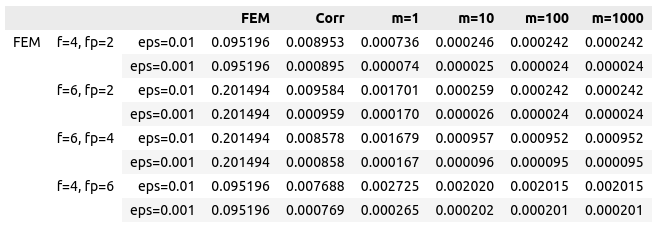
\includegraphics[width=\linewidth]{erreur.png}
	\end{minipage}
	\begin{minipage}{0.48\linewidth}
		\centering
		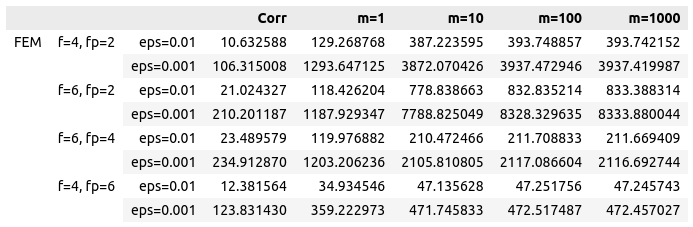
\includegraphics[width=\linewidth]{facteur.png}
	\end{minipage}
	
	\begin{minipage}{\linewidth}
		\centering
		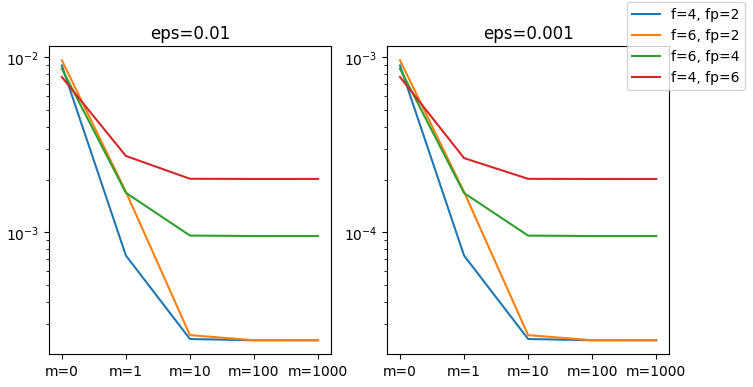
\includegraphics[width=0.6\linewidth]{courbes.png}
	\end{minipage}

	\section*{Application à $\phi$-FEM}
	
	On souhaitera par la suite obtenir le même type de résultats avec $\phi$-FEM. L'idée décrite ici sera la même mais pour l'instant les résultats obtenus ne sont pas ceux attendus.
	
\end{document}